\chapter{Software-arkitektur}

I projektet blev det valgt at lave hjemmesiden i ASP.NET MVC. I følgende afsnit redegøres for systemets arkitektur og de anvendte patterns sammen med en begrundelse for deres valg.

\section{ASP.NET}
ASP.NET er et udviklings framework for web-applikationer.
Det er en del af .NET Frameworket, der gør at al kode, der er  kompatible med .NET og CLR også er kombatibelt i ASP.NET. Dette har været en af de væsentligste grunde til, at ASP.NET er blevet benyttet, da det har gjort at projektet kunne skrives i C\#, der er blevet undervist i på semesterets andre kurser. Gruppen har desuden også modtaget undervisning i ASP.NET i forbindelse med faget I4GUI.

\section{MVC}
Model-View-Controller\cite{MVC} er et GUI-pattern, der forsøger at adskille den grafiske brugergrænseflade fra resten af systemet. Denne adskille gør, at applikationen bliver mere testbar og samtidig mere skalerbar.
MVC består af 3 dele:
\begin{itemize}
	\item Model: er den domænespecifikke kode, der indeholder klasserne og den tilhørende kode for ens application.
	\item View: er den grafiske del af programmet og indeholder præsentationslogikken.
	\item Controller:er en grænsefladen mellem modellen og viewet. Dens opgave er at opdatere brugergrænsefladen og modellen.
\end{itemize}

MVC blev valgt på baggrund af, at det er en integreret del af ASP.NET MVC. ASP.NET MVC er sat op en måde så applikationen bliver router rundt på baggrund af argumenterne i url.
Dette bliver sat op i RouteConfig.cs, hvor der som standard er følgende opsætning:
\begin{verbatim}
public class RouteConfig
{
	public static void RegisterRoutes(RouteCollection routes)
	{
		routes.IgnoreRoute("{resource}.axd/{*pathInfo}");
		
		routes.MapRoute(
		name: "Default",
		url: "{controller}/{action}/{id}",
		defaults: new { controller = "Home", action = "Index", id = UrlParameter.Optional }
		);
	}
}
\end{verbatim}
Overordnede kode viser, hvordan ASP.NET MVC router mellem de forskellige sider på baggrund af url'en. Det første argument i url'en er controlleren, der tager stilling til, hvilken controller, der skal kaldes. Næste argument er actionen, der skal kaldes i den valgte controller og det sidste argument er parametrene actionen skal kaldes med.
Det kan også ses, at der er opsat nogen default argumenter, hvis der ikke er angivet nogen.

\section{Lag}
Systemet bygger på en trelagsmodel som kan ses i figur \ref{fig:lagmodel}.
\begin{figure}[H]
	\centering
	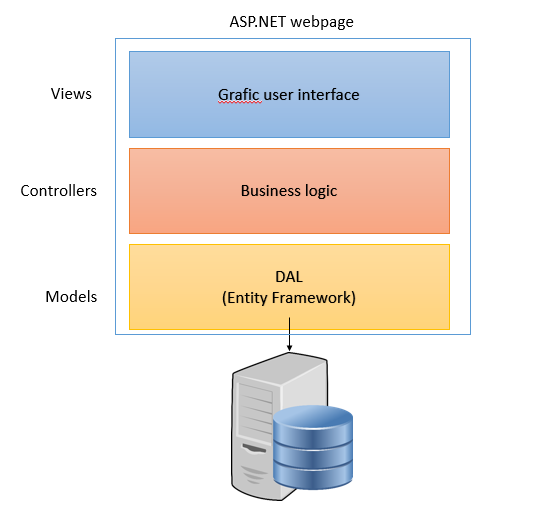
\includegraphics
	[width=165mm]{figures/lagmodel.png}
	\caption{Lagmodel for systemet}
	\label{fig:lagmodel}
\end{figure}

Hvis man lægger denne model ned over systemet, kan man sige at Viewet er præsentationslogikken, controllers og modellen er business logikken og entity framework samt modellen er vores Data access lag.

\subsection{Presentationlag}
For et system som dette, og med de ikke-funktionelle krav der er stillet, er brugervenlighed i højsædet. Dette betyder at præsentationslogikken er ekstremt vigtig for systemet. Det skal være let for en bruger at navigere rundt på siden og kunne forstå hvad meningen er med de forskellige handlinger der kan foretages.

Da projektet er en webapplikation præsenteres den grundlæggende i HTML i en given browser. Denne HTML bliver vha. CSS og Javascript stylet så udseendet bliver godt at se på som muligt. I forbindelse med styling af views er front-end frameworket Bootstrap\cite{Bootstrap} anvendt. Bootstrap bliver anvendt på mange hjemmesider, og er derfor en stor hjælp til let at lave et velkendt design.

I  praksis bliver  præsentationslaget i ASP.NET returneret i controllers. Disse controllers foretager en handling med fx et databasekald, hvorefter der returneres et view fra controlleren som brugeren kan se.
\subsection{Businesslag}
Businesslaget i projektet ligger i høj grad i controllerne. Der er selvfølgelig også truffet nogle forretningsspecifikke valg i Modellen, men dette er primært tomme entiteter. Forretningslogikken ligger derfor som udgangspunkt i controllerne, forsøgt afkoblet så meget som muligt fra præsentationslaget, hvor der helst ikke skal ligge for meget logik. I ASP.NET MVC sender man ofte data til viewet fra controlleren i et enkelt objekt, for bedst at kunne arbejde parallelt med views i mens forretningslogikken bliver implementeret. Derfor går en del af forretningslogikken også udpå at fremstille eller samle et objekt der har et klart interface til at kunne blive anvendt i viewet. 

\subsection{Databaselag}
I BargainBarter anvendes ADO.Net Entity Framework\cite{ADOEF} som det nederste data access layer. Entity Framework er et stærkt framework der har potentialet til at fjerne det impedans mismatch der ofte opstår mellem en database og objektmodellenn i et projekt. Entity Framework er valgt da man vha. en objekt orienteret tankegang kan operere på en database, og derfor slipper for en del bekymringer og ekstraarbejde man ellers vil have. I brugen af Entity Framework har LINQ \cite{LINQ} været et godt supplement det at operere på databasen. 

Entity Framework var desuden en oplagt mulighed, da der i projektet har været stillet en Microsoft SQL Server Database til rådighed som Entity Framework arbejder bedst på. Udover dette arbejder Entity Framework også godt sammen med ASP.Net MVC frameworket.  

I brugen af Entity Framework, anvendes en Code First New Database\cite{EFCodeFirst} approach. På denne måde bliver databasen genereret på baggrund af objektmodellen man opstiller i projektet, og man kan via migrations gemme på historikken på databasen. Denne approach er derfor meget fleksibel idet man altid kan rulle databasen tilbage til et tidligere stadie hvis man fortryder. Fordi man uddelegerer mapningen mellem objektmodellen og entitetsmodellen til et framework, med nogle meget strikse regler kommer disse to forskellige modeller til at ligne hinanden og interfacet fra projektet til databasen bliver derfor meget homogent og let anvendeligt. 

Dette er derfor også nogen af grundene til at beslutningen om at anvende Entity Framework blev truffet tidligt i projektet, og i høj grad har indflydelse på arkitekturen.

\section{Repository Pattern}
Repository er et pattern, der indføres et ekstra lag (Repository-lag), der virker som DAL mellem buisness-logikken og det oprindelige DAL - i dette tilfælde Entity Framework. Dette medfører at buisness-logikken ikke skriver direkte ned i databasen, så dette ikke bliver afhængig af databasen. Buisness-laget kalder bare ned i repository-laget, der så sørger for transaktionen med databasen. 
Repository pattern er blevet anvendt for at opnå en lavere kobling i systemet mellem databasen og buisness-logikken. Den lavere kobling gør systemet mere robust for ændre og gør samtidig også, at man kan teste på, at buisness-logikken der skal skrive ned i databasen. Da man kan stubbe/mocke repository-laget ud.

\section{Unit Of Work}
Unit of Work er et design pattern, der holder styr på in-memory opdateringer og skriver disse opdateringer til databasen. Dette er dermed den eneste klasse, der taler sammen med databasen.
Dette er blevet opnået ved at, at unitofWork-klassen indeholder et GenericRepository af alle de forskellige model-klasser. Det er unitofwork, der vedligeholder disse repositories, da unitofwork er den eneste, der tilføjer eller sletter i databasen. Det er dermed unitofwork, der laver de gængse database-transaction og sørge for at databasen bliver opdateret, når en transaction er færdig.

\section{SignalR}
SignalR er et biblotek til ASP.NET miljøet, som giver adgang til at benytte real-time funktioner på det website man udvikler på. Det er meget nyttigt, når man vil have en form for interaktion med brugerne, eller mellem brugere. Det forgår i browseren, men kan stadig lave kald tilbage til severen. 
\section{Generelle overvejelser i forbindelse med Arkitektur}